% \todo[inline]{After exams - better usage of space - two screenshots next to each other - a pair for each app except profile editor}
\section{Wireframes}
Let's now look at what the users of our application will see.
\autoref{guest-profile-eitor-mockup} contains a mockup of the guest profile editor application.
On the screen, the guest can see what their dietary profile currently contains.
There are controls for adding information to the profile and for saving it.

\begin{figure}[h]
  \centering
  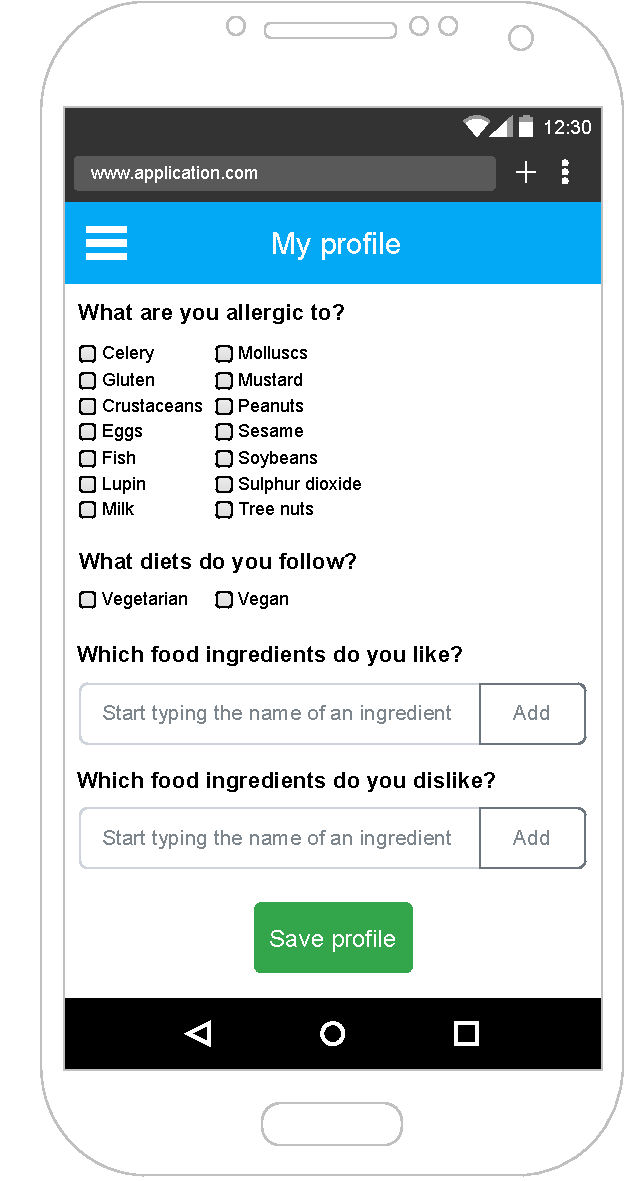
\includegraphics[width=0.4\linewidth]{master-thesis/img/wireframes/dietary_profile_editor.pdf}
  \caption{The guest profile editor application}\label{guest-profile-eitor-mockup}
\end{figure}

\autoref{restaurant-menu-maker-overview-mockup} shows what will the restaurant employee see when they log in to the restaurant menu maker application.
The screen contains a list of previously created menus by the restaurant employee.
Each menu has buttons to view, edit and delete the menu.
There is also a button for creating a new menu.

\begin{figure}[h]
  \centering
  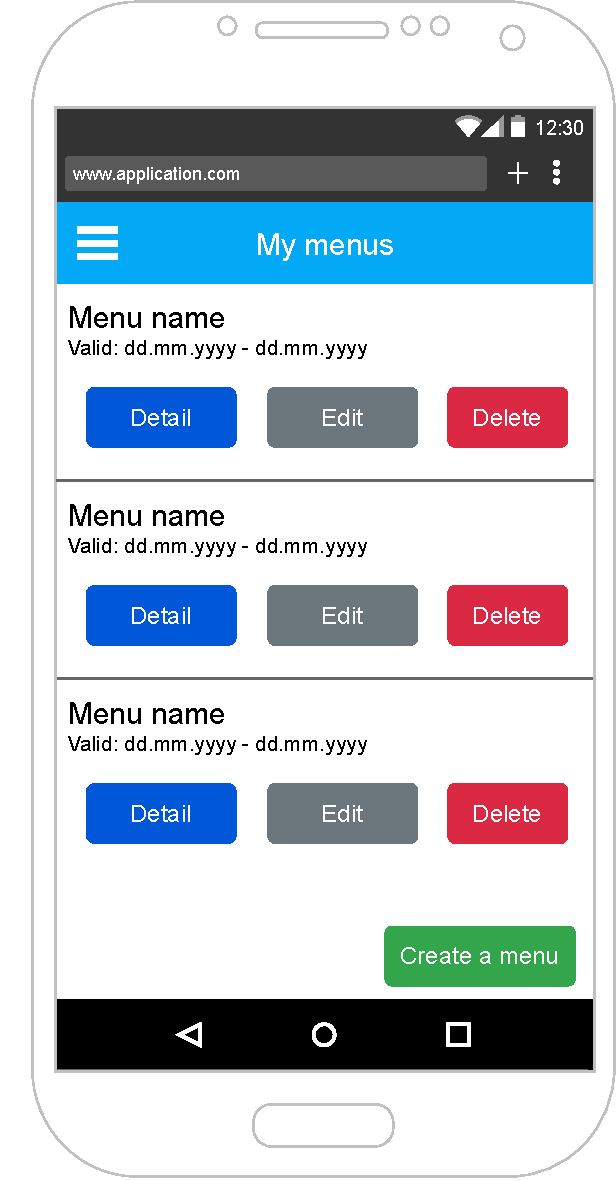
\includegraphics[width=0.4\linewidth]{master-thesis/img/wireframes/menu_creator_menus_overview.pdf}
  \caption{The menus overview screen of the restaurant menu maker application}\label{restaurant-menu-maker-overview-mockup}
\end{figure}

\autoref{restaurant-menu-maker-new-menu-mockup} contains a mockup of the screen which is displayed when a restaurant employee is creating a new menu.
There are fields for specifying the menu's name and date of validity.
A guest can use buttons for adding a category, an existing item or a new item to the menu.

% \todo[inline]{After exams - add categories to menus - a user can click inside the menu to add categories and items to these categories}
\begin{figure}[h]
  \centering
  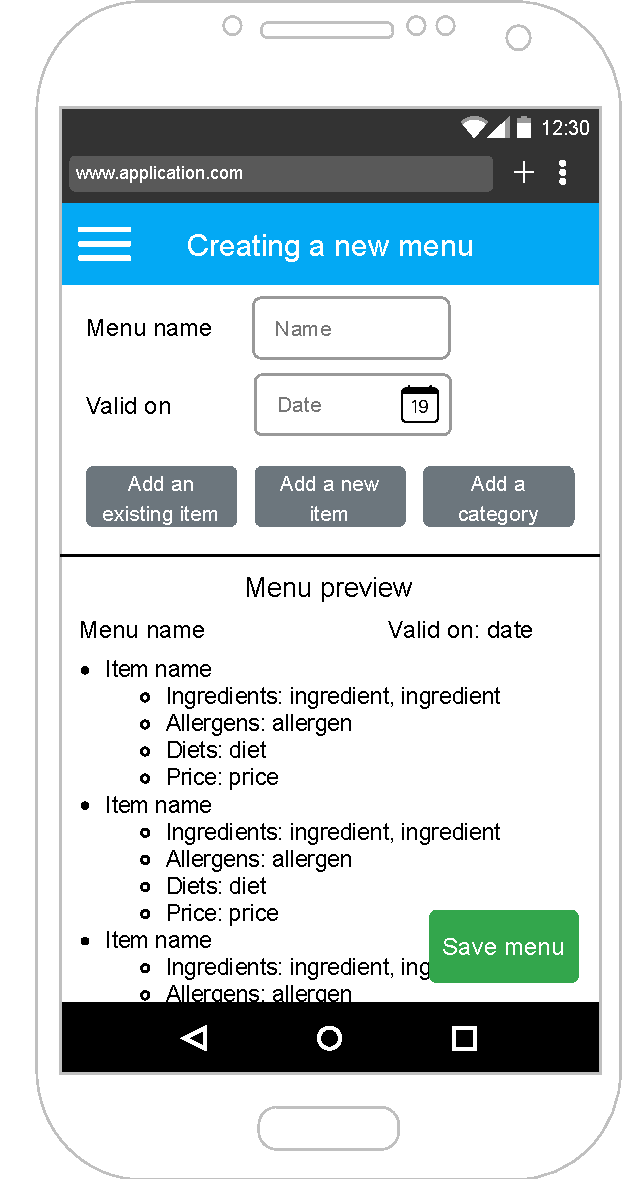
\includegraphics[width=0.4\linewidth]{master-thesis/img/wireframes/menu_creator_new_menu.pdf}
  \caption{The new menu screen of the restaurant menu maker application}\label{restaurant-menu-maker-new-menu-mockup}
\end{figure}

\autoref{guest-menu-viewer-currently-served-mockup} shows a screen which is displayed when a restaurant guest logs in to the personalized menu viewer application.
The screen contains an overview of currently served foods by the guest's favorite restaurants.
A restaurant's name is a clickable link which takes the guest to the restaurant's detail.

\begin{figure}[h]
  \centering
  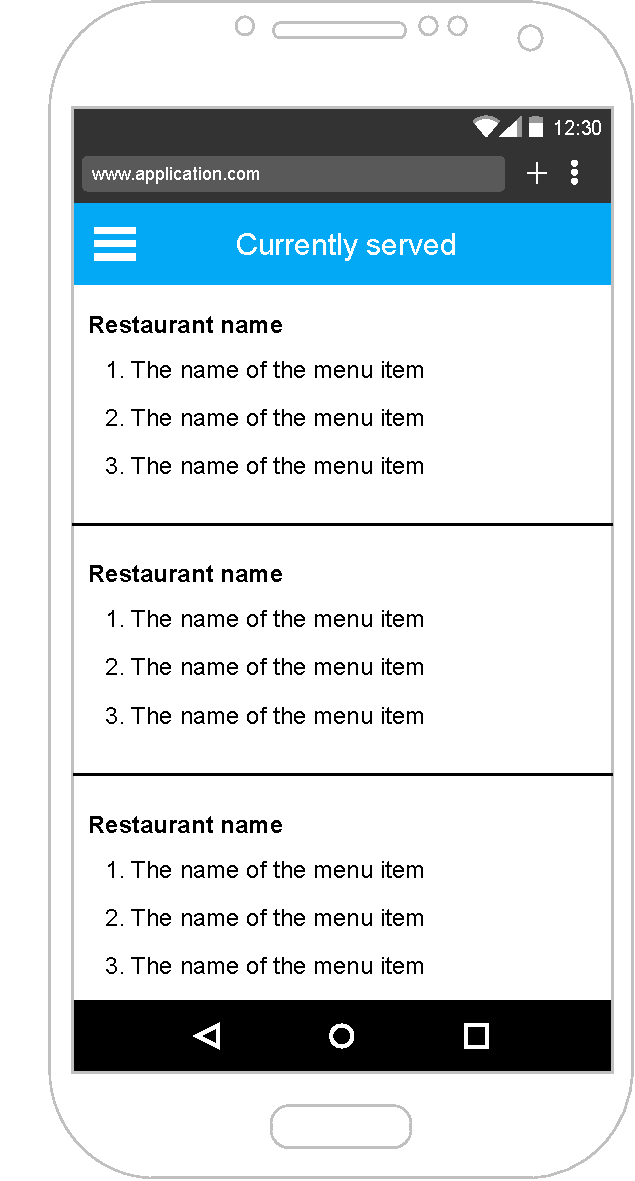
\includegraphics[width=0.4\linewidth]{master-thesis/img/wireframes/menu-viewer-currently-served.pdf}
  \caption{The personalized menu viewer application's home page}\label{guest-menu-viewer-currently-served-mockup}
\end{figure}

A detail of a menu can be seen in \autoref{guest-menu-viewer-menu-detail-mockup}.
The menu is divided into two sections.
The first section contains the items which the guest can eat.
The second section contains the items which the guest cannot eat and within each item, the reason why the guest should avoid the food is highlighted, e.g. that it contains a certain allergen which the guest is allergic to.

\begin{figure}[h]
  \centering
  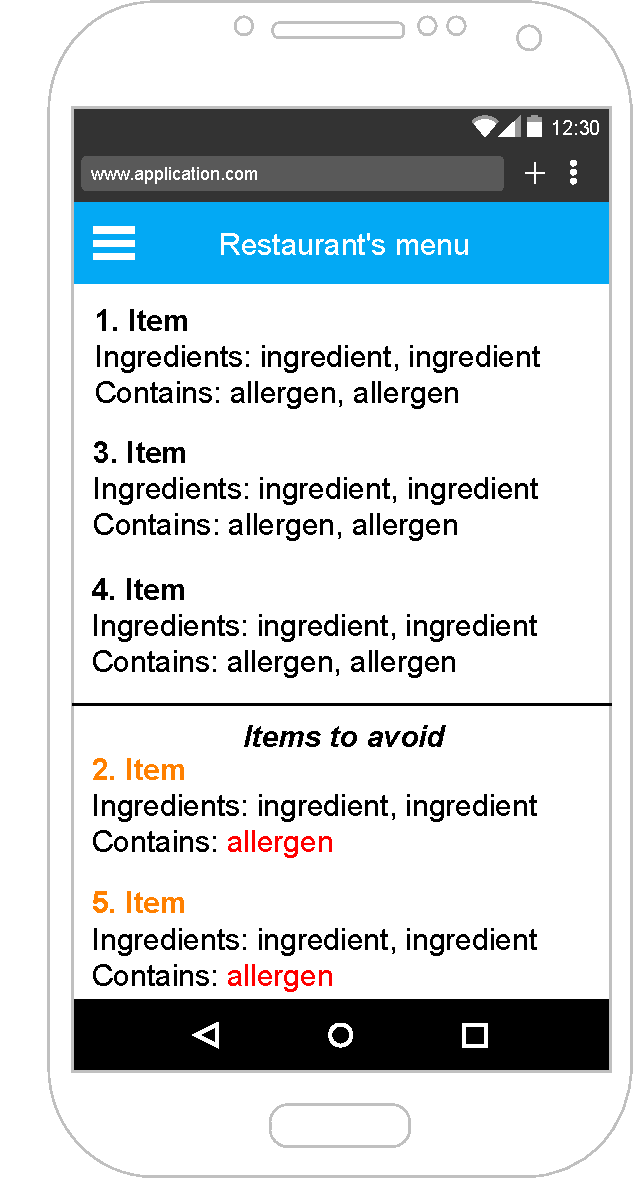
\includegraphics[width=0.4\linewidth]{master-thesis/img/wireframes/menu_viewer_menu_detail.pdf}
  \caption{The personalized menu viewer application's menu detail}\label{guest-menu-viewer-menu-detail-mockup}
\end{figure}
